% !TEX encoding = UTF-8
% !TEX TS-program = pdflatex
% !TEX root = Appunti.tex

\thispagestyle{empty}

\begin{multicols}{2}
\vspace*{120pt}
\begin{figure}[H]
	\centering
	% Sono distribuite tre immagini, 
	% decommentate quella che preferite e lasciate commentate le altre: 
	
	% A colori non compressa:
%	\includegraphics[width=0.99\columnwidth]{Immagini/MotherNature.png}
	% In bianco e nero compressa:
%	\includegraphics[width=0.99\columnwidth]{Immagini/MotherNaturebw.png}
	% A colori compressa:
	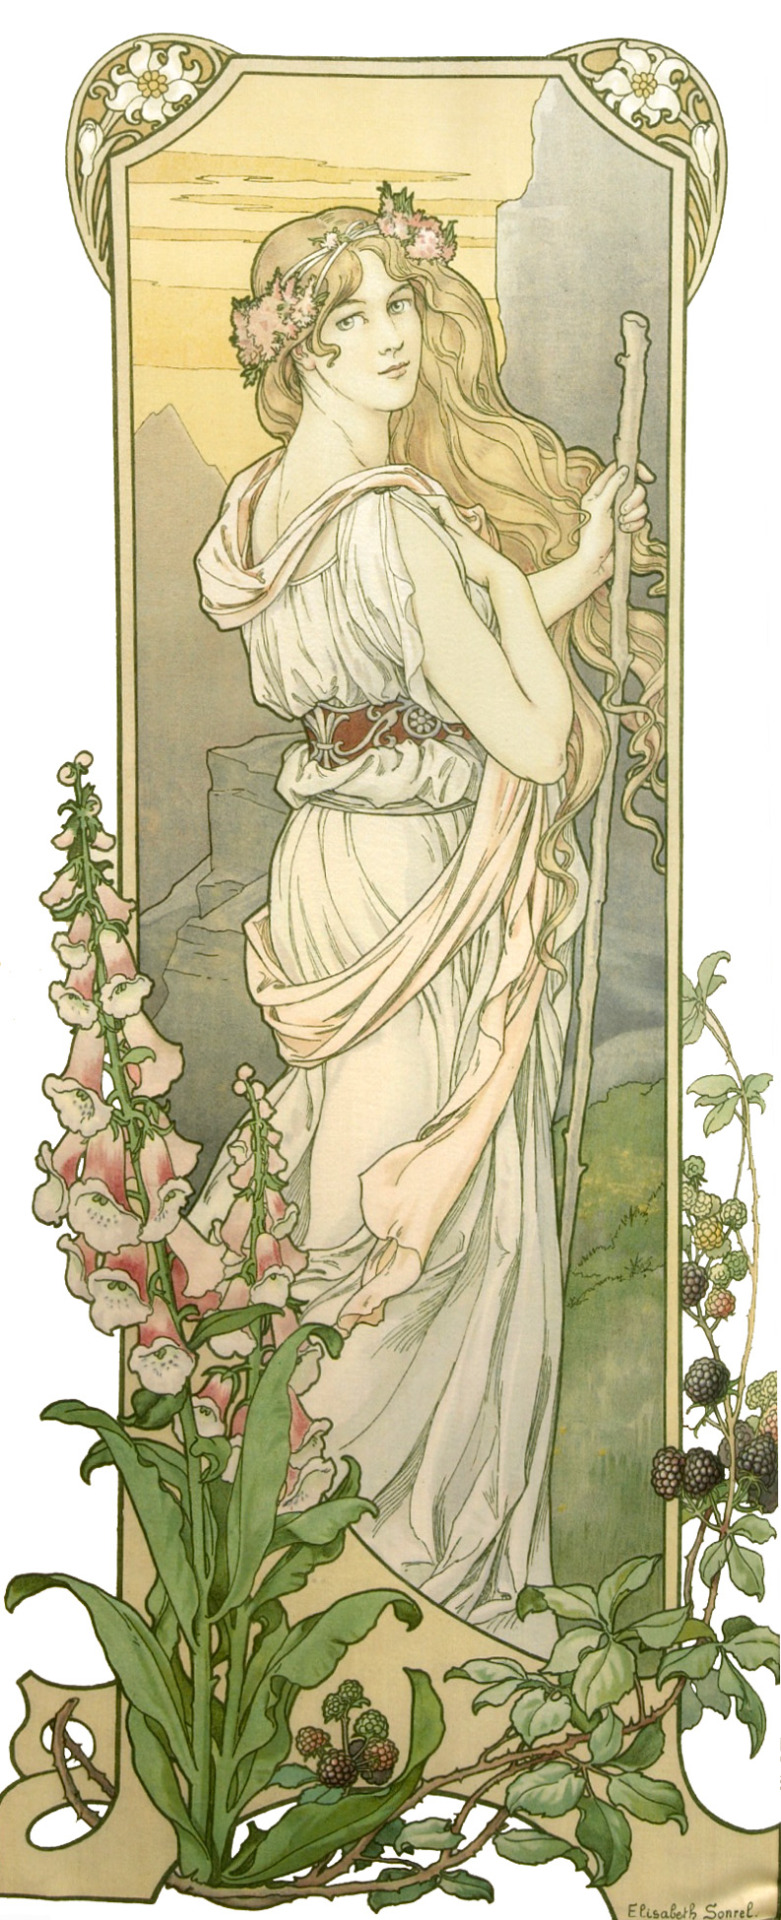
\includegraphics[width=0.99\columnwidth]{Immagini/MotherNaturecompress.png}
\end{figure}

\vfill\null
\columnbreak

\begin{flushright}
	\vspace*{100pt}
	{\fontfamily{lmr}\fontshape{bs}\fontsize{2cm}{1.5cm}\selectfont
		 Struttura \\della \\Materia}\\
	\vspace{20pt}
	{\fontfamily{lmr}\fontshape{it}\fontsize{0.8cm}{0cm}\selectfont Alessandro Candido}\\
\end{flushright}
\vspace{30pt}
\end{multicols}